%
% This is a borrowed LaTeX template file for lecture notes for CS267,
% Applications of Parallel Computing, UCBerkeley EECS Department.
% Now being used for CMU's 10725 Fall 2012 Optimization course
% taught by Geoff Gordon and Ryan Tibshirani.  When preparing 
% LaTeX notes for this class, please use this template.
%
% To familiarize yourself with this template, the body contains
% some examples of its use.  Look them over.  Then you can
% run LaTeX on this file.  After you have LaTeXed this file then
% you can look over the result either by printing it out with
% dvips or using xdvi. "pdflatex template.tex" should also work.
%

\documentclass[twoside]{article}
\setlength{\oddsidemargin}{0.25 in}
\setlength{\evensidemargin}{-0.25 in}
\setlength{\topmargin}{-0.6 in}
\setlength{\textwidth}{6.5 in}
\setlength{\textheight}{8.5 in}
\setlength{\headsep}{0.75 in}
\setlength{\parindent}{0 in}
\setlength{\parskip}{0.1 in}

%
% ADD PACKAGES here:
%

\usepackage{amsmath,amsfonts,graphicx}

%
% The following commands set up the lecnum (lecture number)
% counter and make various numbering schemes work relative
% to the lecture number.
%
\newcounter{lecnum}
\renewcommand{\thepage}{\thelecnum-\arabic{page}}
\renewcommand{\thesection}{\thelecnum.\arabic{section}}
\renewcommand{\theequation}{\thelecnum.\arabic{equation}}
\renewcommand{\thefigure}{\thelecnum.\arabic{figure}}
\renewcommand{\thetable}{\thelecnum.\arabic{table}}

%
% The following macro is used to generate the header.
%
\newcommand{\lecture}[4]{
   \pagestyle{myheadings}
   \thispagestyle{plain}
   \newpage
   \setcounter{lecnum}{#1}
   \setcounter{page}{1}
   \noindent
   \begin{center}
   \framebox{
      \vbox{\vspace{2mm}
    \hbox to 6.28in { {\bf EE302 - Feedback Systems
	\hfill Spring 2019} }
       \vspace{4mm}
       \hbox to 6.28in { {\Large \hfill Lecture #1 \hfill} }
       \vspace{2mm}
       \hbox to 6.28in { {\it Lecturer: #2 \hfill } }
      \vspace{2mm}}
   }
   \end{center}
   \markboth{Lecture #1}{Lecture #1}

   \vspace*{4mm}
}
%
% Convention for citations is authors' initials followed by the year.
% For example, to cite a paper by Leighton and Maggs you would type
% \cite{LM89}, and to cite a paper by Strassen you would type \cite{S69}.
% (To avoid bibliography problems, for now we redefine the \cite command.)
% Also commands that create a suitable format for the reference list.
\renewcommand{\cite}[1]{[#1]}
\def\beginrefs{\begin{list}%
        {[\arabic{equation}]}{\usecounter{equation}
         \setlength{\leftmargin}{2.0truecm}\setlength{\labelsep}{0.4truecm}%
         \setlength{\labelwidth}{1.6truecm}}}
\def\endrefs{\end{list}}
\def\bibentry#1{\item[\hbox{[#1]}]}

%Use this command for a figure; it puts a figure in wherever you want it.
%usage: \fig{NUMBER}{SPACE-IN-INCHES}{CAPTION}
\newcommand{\fig}[3]{
			\vspace{#2}
			\begin{center}
			Figure \thelecnum.#1:~#3
			\end{center}
	}
% Use these for theorems, lemmas, proofs, etc.
\newtheorem{theorem}{Theorem}[lecnum]
\newtheorem{lemma}[theorem]{Lemma}
\newtheorem{proposition}[theorem]{Proposition}
\newtheorem{claim}[theorem]{Claim}
\newtheorem{corollary}[theorem]{Corollary}
\newtheorem{definition}[theorem]{Definition}
\newenvironment{proof}{{\bf Proof:}}{\hfill\rule{2mm}{2mm}}

% **** IF YOU WANT TO DEFINE ADDITIONAL MACROS FOR YOURSELF, PUT THEM HERE:

\begin{document}

% Lecture Details
\lecture{4}{Asst. Prof. M. Mert Ankarali}

\par 

\section{Block Diagrams \& Simplifications}

\subsection{Fundamental Block Diagram Topologies} 

\textbf{Cascaded (Series) Block Diagrams}

  \begin{minipage}[h]{0.6\linewidth}
    \begin{center}
      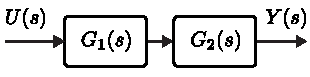
\includegraphics[width=0.85\textwidth]{cascade}
    \end{center}
  \end{minipage}
  \begin{minipage}[h]{0.4\linewidth}
    \begin{center}
      \begin{align*}
      \frac{Y(s)}{U(s)} = \bar{G}(s) = G_1(s) G_2(s)
       \end{align*}
    \end{center}
  \end{minipage}
  
  \textbf{Parallel Block Diagrams}
  
    \begin{minipage}[h]{0.6\linewidth}
    \begin{center}
      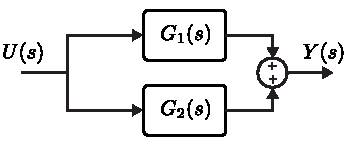
\includegraphics[width=1\textwidth]{par}
    \end{center}
  \end{minipage}
  \begin{minipage}[h]{0.4\linewidth}
    \begin{center}
      \begin{align*}
      \frac{Y(s)}{U(s)} = \bar{G}(s) = G_1(s) + G_2(s)
       \end{align*}
    \end{center}
  \end{minipage}
  
\textbf{Negative Feedback Loop}

    \begin{minipage}[h]{0.6\linewidth}
    \begin{center}
      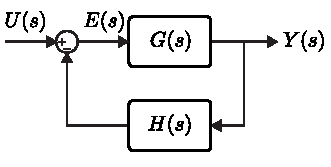
\includegraphics[width=0.95\textwidth]{feedback}
    \end{center}
  \end{minipage}
  \begin{minipage}[h]{0.4\linewidth}
    \begin{center}
      \begin{align*}
      &E(s) = U(s) - H(s) Y(s)
      \\
      &E(s) \left(1 + H(s) G(s) \right) = U(s) 
      \\
      &\frac{Y(s)}{U(s)} = \bar{G}(s) = \frac{G(s)}{1 + H(s) G(s)}
       \end{align*}
    \end{center}
  \end{minipage}
  
  \newpage
  
  \subsection{Examples} 
  
  \textbf{Ex 1:} Simplify the following block-diagram topology
  
      \begin{minipage}[t]{0.95\linewidth}
    \begin{center}
      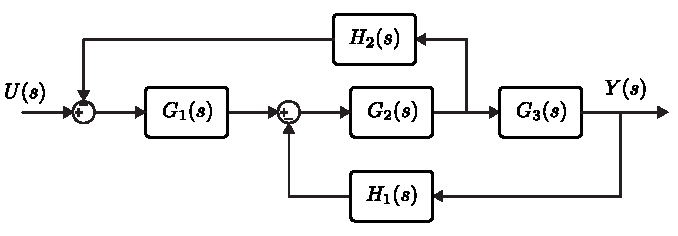
\includegraphics[width=0.55\textwidth]{ex1}
    \end{center}
  \end{minipage}
  
\textbf{Solution:} 
  
        \begin{minipage}[h]{0.95\linewidth}
    \begin{center}
      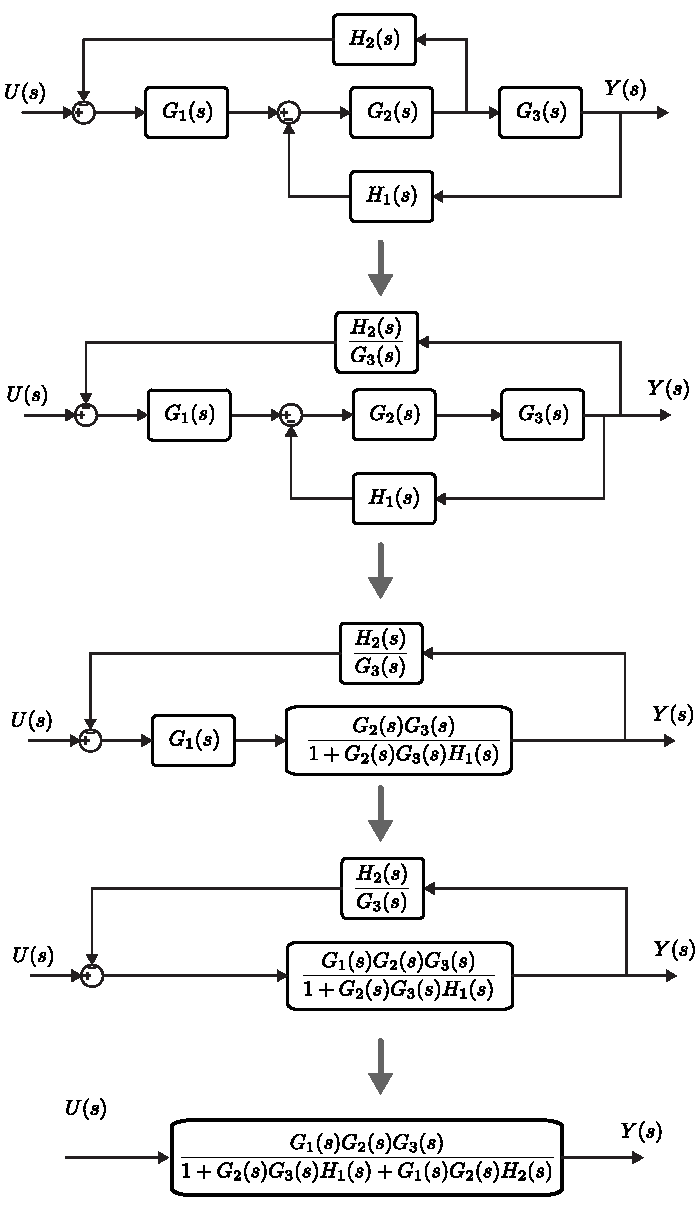
\includegraphics[width=0.55\textwidth]{ex1_sol}
    \end{center}
  \end{minipage}
  
% **** This ENDS THE EXAMPLES. DON'T DELETE THE FOLLOWING LINE:
\end{document}